\subsection{Ablation Study}
% In this section, we analyze the effectiveness and efficiency of \workname from three aspects: supervision information, training cost, and pre-training datasets. 
% If not mentioned, hyper-parameters, image encoder and text encoder are kept the same as ResNet50 in the section \ref{Training Setup}. 


\begin{table}
	\begin{minipage}{0.48\linewidth}
		\caption{Ablation on additional supervision. SS/MVS/NNS denotes Self-Supervision, Multi-View Supervision and Nearest-Neighbor Supervision, respectively.}
		\label{tab:ablation on supervision information}
		\centering
		\footnotesize
		\resizebox{\textwidth}{!}{
        \begin{sc}
        \begin{tabular}{cccccccc}
        \toprule
         \textbf{CLIP} & \textbf{MVS} & \textbf{SS} & \textbf{NNS} & \textbf{Zero-shot}  \\
        \midrule
          \checkmark &$\times$&$\times$&$\times$& 20.6\\
          \checkmark & \checkmark &$\times$&$\times$& 24.8($\uparrow$ +4.2)\\
          \checkmark & \checkmark & \checkmark &$\times$  & 25.4($\uparrow$ +4.8)\\
          \checkmark & \checkmark & \checkmark & \checkmark & \textbf{27.2($\uparrow$ +6.6)}\\
        \bottomrule
        \end{tabular}
        \end{sc}}
	\end{minipage}\hfill
	\begin{minipage}{0.5\linewidth}
		\centering
		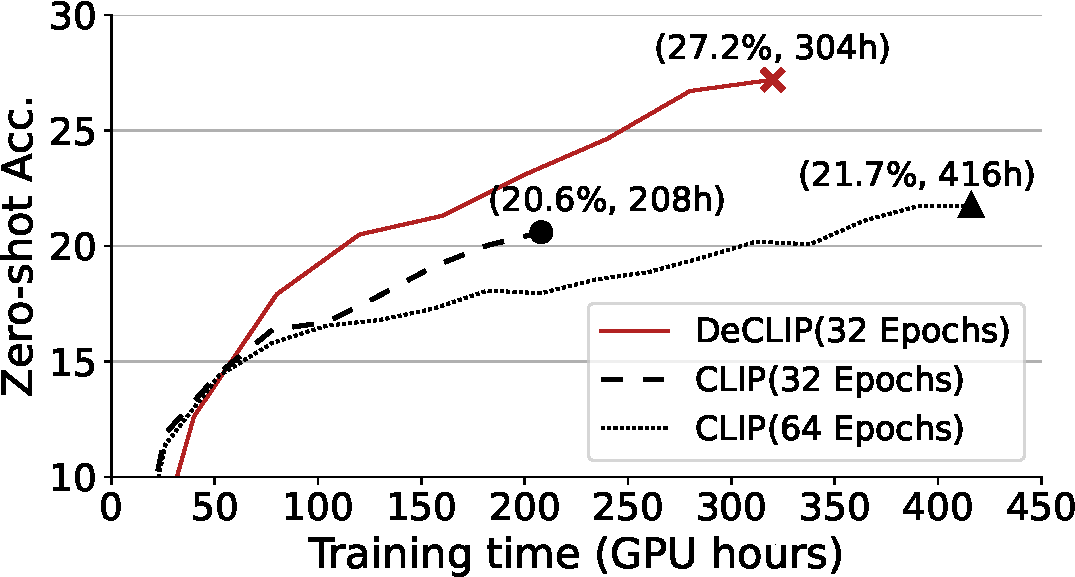
\includegraphics[width=0.99\columnwidth]{DeCLIP/figs/Result_CC.pdf}
		\captionof{figure}{Ablation on pre-training cost on CC3M dataset. The proposed method performs better with less training time.}
		\label{fig:abl_training_time}
	\end{minipage}
	\vspace{-2em}
\end{table}

\paragraph{Ablation on additional supervision}
In order to understand the effectiveness of each additional supervision, we conduct an ablation study as indicated in Tab.~\ref{tab:ablation on supervision information}. We follow the \workname-ResNet50 protocol in the pre-training setup except for a smaller 1024 batch size on a smaller CC3M dataset. The single image-text contrastive supervision (CLIP) results in 20.6\% zero-shot top1 accuracy on ImageNet. We can observe that MVS boost amazing 4.2\% improvement over the original CLIP. As discussed in Sec.~\ref{sec:mvs}, the benefits might come from two sides: 1). the MVS can look at a small local view of an image which might be a better fit with the text description. 2). $2\times2$ augmented views can provide $3\times$ diverse and high-quality additional supervision, thus leading to more robust representations. SS can further contribute an additional 0.6\% improvement on the basis of MVS. We believe SS could bring more improvements with proper dedicated SSL methods. NNS further brings 1.8\% improvement on the high basis of SS. We will discuss more about NNS at Sec.~\ref{sec:nn_samples}. On the YFCC15M dataset, our \workname using full additional supervision gets significant effect improvement, Appendix~\ref{Additional study} shows the details.

% We study the performance of \workname from the perspective of more supervised information on CC3M setting. As shown in Tabel \ref{tab:ablation on supervision information}, we show the zero-shot top1 accuracy on ImageNet with incremental supervision information. Row 1 of Tabel \ref{tab:ablation on supervision information} shows baseline and specific supervision method, of which baseline is the naive contrastive between image and text,
% MVS means using the augmentation to get two views, SS means image and language self-supervision within its own modality, NNS is text nearest neighbor supervision in a mini-batch.  
% Row 2-5 of Tabel \ref{tab:ablation on supervision information} shows the significant results of our approach in CC3M datatset. We can observe that MVS get 4.2\% improvement on zero-shot ImageNet top1 accuracy, which is the most contribution in the three parts of DeCLIP. SS contributes additional 0.6\% improvement on the basis of multi-view supervision. NNS also brings objective improvement of 1.6\% on the basis of SS. In addition, we sample some NNS example, as shown in Fig.~\ref{fig:nn_figure}, the first line is the original image-text pairs, and the second line is the extra image-text pairs found through NNS. We can intuitively see that these two texts are indeed highly similar in meaning, and both can be used as the description of first line images, which proves that NNS is reasonable.


% We also train full setups of \workname on the YFCC15M dataset to compare the results of CLIP. Tabel \ref{tab:ablation on YFCC} is the comparison result of our approach and CLIP zero-shot top1 accuracy on ImageNet, using the same encoder and training data size. We can see that the 41.9\% zero-shot of \workname compare to zero-shot 35.9\% of reproduced CLIP, which is an amazing 6.0\% improvement on the YFCC15M dataset. In addition, we use the linear probe method to evaluate the pre-training model, which is trained on YFCC15M dataset, on the Fowers, Stanford Cars and ImageNet datasets. It can be seen from Table \ref{tab:YFCC downstream result} that our approach has 2.0\% improvement on the Fowers, 5.5\% improvement on the Stanford Cars, and 5.5\% improvement on the ImageNet. It is worth noting that the zero-shot we reproduced is higher than the report of CLIP, but the linear probe is lower than the report. This may be due to YFCC15M dataset differences. In addition, we use more stringent text cleaning rules to get high quality text, this will improve the zero shot ability, but may not improve the pre-training ability. Overall, \workname exceeds reported CLIP both zero-shot result and linear probe result on the YFCC15M dataset. This result further proves the strong generalization ability of our paradigm.






% \begin{table*}[h]
% \caption{\label{tab:ablation on YFCC} \workname Zero-Shot performance of ImageNet Top1 on YFCC datasets.}
% \label{sample-table}
% \begin{center}
% \begin{small}
% \begin{sc}
% \begin{tabular}{cccccc}
%   \toprule  
%   %\multicolumn{5}{r}{}  \\
%   \textbf{Model} &\textbf{Backbone} & \textbf{Dataset}   & \textbf{Data Size}   &\textbf{Batch Size}  & \textbf{Zero-Shot} \\
%   \midrule   
%   CLIP &ResNet50 &YFCC               &15M  & — &31.3 	\\
%   DeCLIP Baseline & ResNet50 &YFCC    &15M  & 4,096 &35.9 \\
%   \textbf{DeCLIP} &\textbf{ResNet50} &\textbf{YFCC} &\textbf{15M}  &\textbf{4,096} &\textbf{41.9(+6.0)} 	\\
%   \bottomrule
% \end{tabular}
% \end{sc}
% \end{small}
% \end{center}
% \end{table*}

% \begin{table*}[h]
% \caption{\label{tab:YFCC downstream result} Linear probe performance on YFCC pre-trained models over 3 datasets.}
% \label{sample-table}
% \begin{center}
% \begin{small}
% \begin{sc}
% \begin{tabular}{ccccc}
% \toprule
% %\rotatebox{90}{Model} & \rotatebox{90}{Backbone}  & \rotatebox{90}{CIFAR10} & \rotatebox{90}{CIFAR100} & \rotatebox{90}{Food101} & \rotatebox{90}{Pets} & \rotatebox{90}{Fowers} & \rotatebox{90}{SUN397} & \rotatebox{90}{Cars} & \rotatebox{90}{DTD} & \rotatebox{90}{Caltech} & \rotatebox{90}{Aircraft} & \rotatebox{90}{ImageNet}    \\
% \textbf{Model} & \textbf{Backbone} &\textbf{Fowers} & \textbf{Stanford Cars}   & \textbf{ImageNet}    \\
% \midrule

% CLIP &ResNet50     & 94.4 & 31.4 & 62.0  \\
% DeCLIP Baseline &ResNet50 &95.0 &26.7 &60.5 \\
% \textbf{DeCLIP}  &\textbf{ResNet50}  & \textbf{97.0(+2.0)} & \textbf{32.2(+5.5)} & \textbf{66.0(+5.5)}\\

% \bottomrule



% \end{tabular}
% \end{sc}
% \end{small}
% \end{center}
% \end{table*}


\paragraph{Ablation on training cost} Since we need to encode twice for each image-text pair, we admit our \workname needs a higher training cost than CLIP. 
Regarding the training time, one \workname iteration equals 1.5$\times$ CLIP iteration. 
In this ablation, we train the original CLIP-ResNet50 longer than our \workname-ResNet50. As shown in Fig.~\ref{fig:abl_training_time}, longer 64 epochs training can bring about 1.1\% improvement. However, our model has 27.2\% top1 accuracy, which is still 5.3\% higher than the time-equivalent CLIP. It reveals that our framework can extract richer and more representative features through our proposed supervision. We also include memory usage ablation in Appendix~\ref{Additional study}.


% \paragraph{\checkme{Ablation on different supervision ratio?}}

% Our \workname uses MVS in training process, it needs to encode twice for each image-text pairs, which increases the training cost. However, since the reading and processing of data in the training process also takes up a large proportion of time-consuming, these only need to be processed once, so the cost brought by MVS is less than 2 times the single view training process. 

% From Figure \ref{fig:cost in YFCC}  we can see that on the YFCC15M dataset, \workname only needs to train 16 epochs to achieve the same top1 accuracy as CLIP training 32 epochs. Considering that the additional cost brought by MVS is less than twice, it can be found that \workname (16epochs) can achieve the same zero-shot top1 accuracy on ImageNet as CLIP when the training cost is less than 32 epochs of CLIP. In actually training, it is found that \workname only needs about 0.7$\times$ training cost to achieve the results reported by CLIP on YFCC15M dataset. In addition, \workname training 32 epochs brings extra cost, but this part of the cost brings a significant 10.6\% improvement, which is almost impossible in CLIP. From Figure \ref{fig:cost in full data}, we can see that on the full dataste, considering that \workname only needs 0.7$\times$ training cost at the same accuracy compared to CLIP, when \workname uses 20 epochs to achieve CLIP 32 epochs accuracy, the training cost required is still slightly less. In addition, \workname can still improve the acuracy when adding more training costs, but CLIP won't. Moreover, the training data used by \workname is 88M and CLIP is 400M, which is 4.5$\times$ less the training costs. Therefore, \workname has achieved better results with less training costs.

% \lf{I think the point here is that naive CLIP models CANNOT reach our accuracy even if they are trained as long as our models. Suppose training our DeCLIP-ResNet50 32epochs equals training CLIP-ResNet50 for 50 epochs, we can just draw a evaluation curve as Fig6. CC-3M is enough. If we can have YFCC, that's much better.}


\subsection{Analysis}

\paragraph{Class activation maps} We try to understand what renders our \workname effective. As shown in Fig.~\ref{fig:attn_vis}, we visualize the class activation maps (CAM)~\citep{zhou2016learning} of different models trained on the YFCC dataset.
% The first row is two cases that both models can have a correct prediction. The CAM of our model segment the complete object, while the CLIP model only looks at a few components. For the second row, where our model performs better than CLIP, the difference becomes more obvious.
The results validate that the proposed method learns more representative features with the aid of multiple supervision.
% We give an intuitive explanation: since our \workname has multi-view supervision, our model is forced to match each view (local region of the whole image) to the representation of the scene. As a result, the representations will be more comprehensive over the image, rather than attend to only a few parts.
% will be informative of the spatial layout and different objects in the image - rather than attend only to the most discriminative image component.
% We compute a weighted sum of the feature maps of the last convolutional layer to obtain our class activation maps. 
\begin{figure}[t]
    \centering
	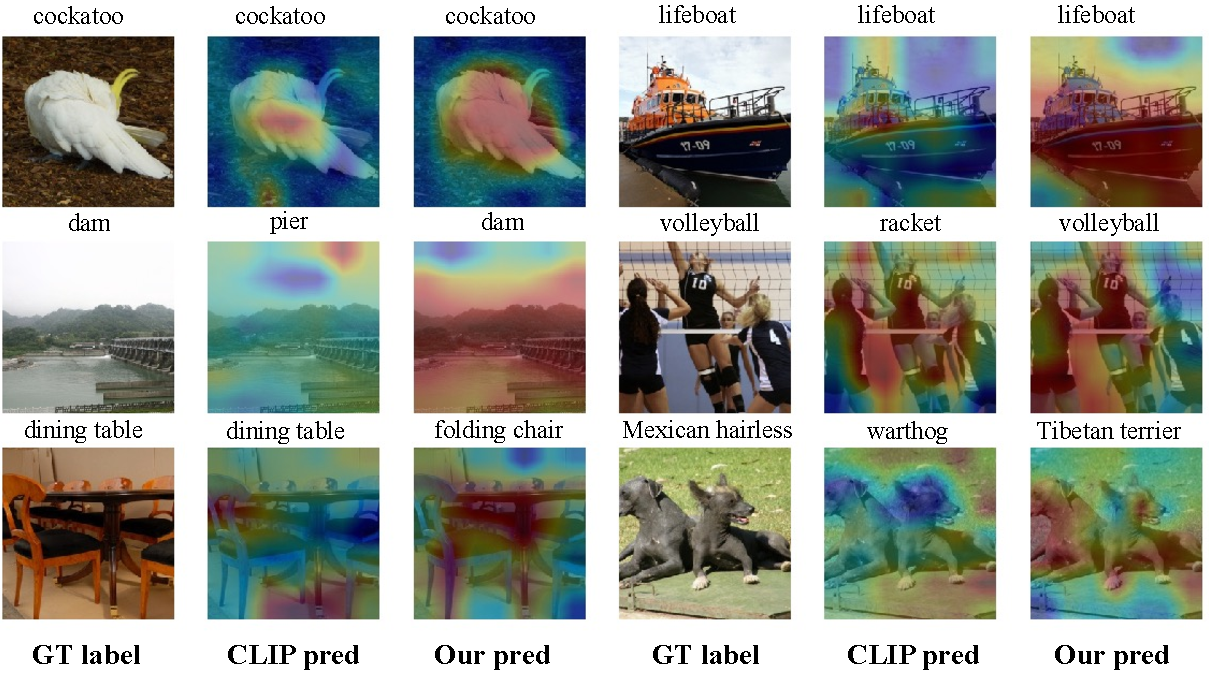
\includegraphics[width=0.7\columnwidth]{DeCLIP/figs/attention_vis.pdf}
	\caption{Class activation maps (CAM) for the CLIP vs. our \workname model trained on the YFCC dataset. The CAMs of our model segment the complete object, while the CLIP model only looks at a few components.}
	\label{fig:attn_vis}
\end{figure}

% \paragraph{Data quality}
\paragraph{Nearest neighbor samples}
\label{sec:nn_samples}
In Fig~\ref{fig:nn_figure}, we show some nearest neighbor (NN) samples from different datasets. The first row is the original image-text pair, while the second row is the NN pair. In general, we can see that the texts have similar intellectual meanings. Therefore, the NN pair can provide high-quality supervision. When taking datasets into consideration, the matching performs very well in well-filtered datasets, such as CC3M and CC12M. This matching might be a little worse in more noisy datasets, such as YFCC and web-crawled, but it can still provide some beneficial guidance.

% the NN pair is similar to the original pair,

% In general, 
% In addition, we sample some NNS example, as shown in Fig.~\ref{fig:nn_figure}, the first line is the original image-text pairs, and the second line is the extra image-text pairs found through NNS. We can intuitively see that these two texts are indeed highly similar in meaning, and both can be used as the description of first line images, which proves that NNS is reasonable.


\begin{figure}[t]
	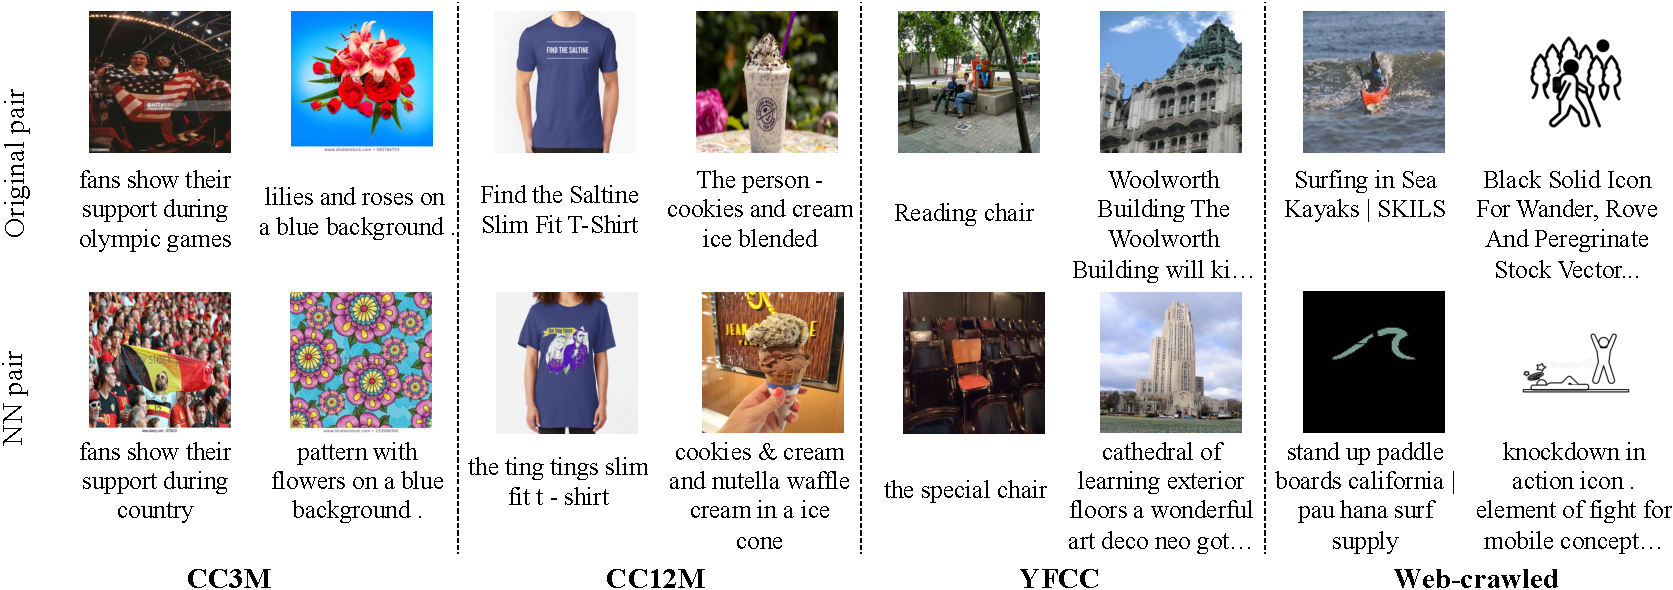
\includegraphics[width=0.99\columnwidth]{DeCLIP/figs/nearest_neighbor_sample.pdf}
    % \vskip -0.15in
	\caption{Nearest neighbor samples from different datasets. As we can see, the NN pair is very similar to the original pair, thus it can provide high-quality supervision. 
	}
	\label{fig:nn_figure}
\end{figure}